\section{Auswertung}
\label{sec:Auswertung}
Zur Auswertung der Messdaten benötigt man den Mittelwert, die Standardabweichung und die Unsicherheit. Dabei gilt
\begin{equation}
  \bar{x}=\dfrac{1}{N}\sum_{i=1}^N x_i
  \label{eq:mean}
\end{equation}
für den Mittelwert $\bar{x}$ einer N-Messungen großen Messreihe der Größe $x$
\begin{equation}
σ=\sqrt{\dfrac{1}{N-1}\sum_{i=1}^N(x_i-\bar{x})^2} 
\label{eq:std} 
\end{equation}
für die Standardabweichung $σ$ und
\begin{equation}
  Δx=\dfrac{σ}{\sqrt{N}}
  \label{eq:unc} 
\end{equation}
für die Unsicherheit $Δx$ der Messgröße $x$. \\

Für eine verknüpfte Messgröße $f(x_1,...,x_N)$ gilt die Gaußsche Fehlerfortpflanzung mit
\begin{equation}
Δf(x_1,...,x_N)=\sqrt{\sum_{i=1}^N (\frac{\partial f}{\partial x_i}Δx_i)^2}
\label{eq:gaussF}
\end{equation}
%T_1 und T_2

\newpage

%Einzelfrequenzen

\subsection{Messung der Einzelfrequenzen}
In \autoref{tab:freiePendel} werden die unabhängigen Periodendauern der beiden Pendel aufgetragen.

\begin{table}[H]
  \centering
  \caption{Periodendauern der einzelnen Pendel}
  \label{tab:freiePendel}
  \sisetup{table-format=1.2}
  \begin{tabular}{S[table-format=2.0] S S[table-format=1.3] S[table-format=2.2] S[table-format=1.3] S[table-format=2.2] S[table-format=1.3] S[table-format=2.2] S[table-format=1.3]}
    \toprule
    \multicolumn{1}{c}{Pendellänge} & \multicolumn{4}{c} {$l= 70 \, \unit{\centi\meter}$} 
    & \multicolumn{4}{c}{$l = 100 \, \unit{\centi\meter}$} \\
    \cmidrule(lr){2-5}\cmidrule(lr){5-9}
    {Messung} & {$5T_1 \mathbin{/} \unit{\second}$} & {$T_1 \mathbin{/} \unit{\second}$} 
    & {$5T_2 \mathbin{/} \unit{\second}$} & {$T_2 \mathbin{/} \unit{\second}$} & 
    {$5T_1 \mathbin{/} \unit{\second}$} & {$T_1 \mathbin{/} \unit{\second}$} 
    & {$5T_2 \mathbin{/} \unit{\second}$} & {$T_2 \mathbin{/} \unit{\second}$}\\
    1 & 8.21 & 1.642 & 8.46 & 1.692 & 9.96  & 1.992 & 9.90  & 1.980 \\
    2 & 8.13 & 1.626 & 8.54 & 1.708 & 9.94  & 1.988 & 10.06 & 2.012 \\
    3 & 8.30 & 1.660 & 8.72 & 1.744 & 9.73  & 1.946 & 9.90  & 1.980 \\
    4 & 8.23 & 1.646 & 8.29 & 1.658 & 9.93  & 1.986 & 9.87  & 1.974 \\
    5 & 8.32 & 1.664 & 8.66 & 1.732 & 10.01 & 2.002 & 9.88  & 1.976 \\
    6 & 8.26 & 1.652 & 8.34 & 1.668 & 10.14 & 2.028 & 10.01 & 2.002 \\
    7 & 8.25 & 1.650 & 8.47 & 1.694 & 9.71  & 1.942 & 9.74  & 1.948 \\
    8 & 8.24 & 1.648 & 8.29 & 1.658 & 10.22 & 2.044 & 9.92  & 1.984 \\
    9 & 8.40 & 1.680 & 8.62 & 1.724 & 9.74  & 1.948 & 10.13 & 2.026 \\
   10 & 8.30 & 1.660 & 8.06 & 1.612 & 9.84  & 1.968 & 9.78  & 1.956 \\
    \bottomrule
  \end{tabular}
\end{table}

Daraus ergeben sich mit \eqref{eq:mean}, \eqref{eq:std} und \eqref{eq:unc}:
\begin{table}[H]
  \centering
  \caption{Mittelwerte, Standardabweichungen und Unsicherheiten der Periodendauern}
  \sisetup{table-format=1.3}
  \begin{tabular}{S S S}
    \toprule
    & {$l=70 \, \unit{\centi\meter}$} & { $l=100 \, \unit{\centi\meter}$} \\
    \midrule
    {$\bar{T}_1$} & 1.653 & 1.984\\
    {$σ_{T_1}$}   & 0.0137 & 0.0327\\
    {$ΔT_1$}      & { \pm 0.014}& {\pm 0.033}\\
    {$\bar{T}_2$} & 1.689 & 1.984 \\
    {$σ_{T_2}$}   & 0.0385 & 0.0227\\
    {$ΔT_2$}      & {\pm 0.038} & {\pm 0.023}\\
    \bottomrule
  \end{tabular}
\end{table}


\newpage

%Gleichphasige Schwingung

\subsection{Gleichphasige Schwingung}
\autoref{tab:GleichphasigeSchwingung} enthält die Messdaten für die gleichphasigie Schwingung.

\begin{table}[H]
  \centering
  \caption{Periodendauern bei der gleichphasigen Schwingung}
  \label{tab:GleichphasigeSchwingung}
  \sisetup{table-format=1.2}
  \begin{tabular}{S[table-format=2.0] S S[table-format=1.3] S[table-format=2.2] S[table-format=1.3]}
    \toprule
    \multicolumn{1}{c}{Pendellänge} & \multicolumn{2}{c} {$l= 70 \, \unit{\centi\meter}$}
    & \multicolumn{2}{c}{$l = 100 \, \unit{\centi\meter}$} \\
    \cmidrule{2-3}\cmidrule{4-5} 
    {Messung} & {$5T_+ \mathbin{/} \unit{\second}$} & {$T_+ \mathbin{/} \unit{\second}$} 
    & {$5T_+ \mathbin{/} \unit{\second}$} & {$T_+ \mathbin{/} \unit{\second}$} \\
    1 & 8.92 & 1.784 & 9.69 & 1.938 \\
    2 & 8.32 & 1.664 & 9.91 & 1.982 \\
    3 & 8.26 & 1.652 & 10.17& 2.034 \\
    4 & 8.68 & 1.736 & 9.79 & 1.958 \\
    5 & 8.54 & 1.708 & 9.80 & 1.960 \\
    6 & 9.13 & 1.826 & 9.81 & 1.962 \\
    7 & 8.04 & 1.608 & 10.15& 2.030 \\
    8 & 8.28 & 1.656 & 9.76 & 1.952 \\
    9 & 8.49 & 1.698 & 9.91 & 1.982 \\
   10 & 8.47 & 1.694 & 9.92 & 1.984 \\
    \bottomrule
  \end{tabular}
\end{table}

Erneut werden Mittelwert, Standardabweichung und Unsicherheit berechnet.

\begin{table}[H]
  \centering
  \caption{Mittelwerte, Standardabweichungen und Unsicherheiten der gleichphasigen Periodendauern}
  \sisetup{table-format=1.3}
  \begin{tabular}{S S S}
    \toprule
    & {$l=70 \, \unit{\centi\meter}$} & { $l=100 \, \unit{\centi\meter}$} \\
    \midrule
    {$\bar{T}_+$} & 1.7025 & 1.9781\\
    {$σ_{T_+}$}   & 0.0619 & 0.0303\\
    {$ΔT_+$}      & {\pm 0.062} & {\pm 0.030}\\
    \bottomrule
  \end{tabular}
\end{table}

\newpage

%Gegenphasige Schwingung

\subsection{Gegenphasige Schwingung}
In Tabelle \autoref{tab:GegenphasigeSchwingung} finden sich die Periodendauern der gegenphasigen Schwingung.

\begin{table}[H]
  \centering
  \caption{Periodendauern bei der gegenphasigen Schwingungen}
  \label{tab:GegenphasigeSchwingung}
  \sisetup{table-format=1.2}
  \begin{tabular}{S[table-format=2.0] S S[table-format=1.3] S[table-format=2.2] S[table-format=1.3]}
    \toprule
    \multicolumn{1}{c}{Pendellänge} & \multicolumn{2}{c} {$l= 70 \, \unit{\centi\meter}$}
    & \multicolumn{2}{c}{$l = 100 \, \unit{\centi\meter}$} \\
    \cmidrule{2-3}\cmidrule{4-5} 
    {Messung} & {$5T_- \mathbin{/} \unit{\second}$} & {$T_- \mathbin{/} \unit{\second}$} 
    & {$5T_- \mathbin{/} \unit{\second}$} & {$T_- \mathbin{/} \unit{\second}$} \\
    1 & 7.10 & 1.420 & 8.83 & 1.766 \\
    2 & 7.16 & 1.432 & 9.24 & 1.848 \\
    3 & 7.85 & 1.570 & 9.37 & 1.874 \\
    4 & 8.07 & 1.614 & 9.11 & 1.822 \\
    5 & 7.60 & 1.520 & 9.44 & 1.888 \\
    6 & 7.74 & 1.548 & 9.18 & 1.836 \\
    7 & 7.55 & 1.510 & 9.40 & 1.880 \\
    8 & 7.70 & 1.540 & 9.13 & 1.826 \\
    9 & 7.83 & 1.566 & 9.47 & 1.894 \\
   10 & 7.72 & 1.544 & 9.17 & 1.834 \\
   \bottomrule
  \end{tabular}
\end{table}

%Unsicherheiten u.s.w.

\begin{table}[H]
  \centering
  \caption{Mittelwerte, Standardabweichungen und Unsicherheiten der gegenphasigen Periodendauern}
  \sisetup{table-format=1.3}
  \begin{tabular}{S S S}
    \toprule
    & {$l=70 \, \unit{\centi\meter}$} & { $l=100 \, \unit{\centi\meter}$} \\
    \midrule
    {$\bar{T}_-$} & 1.526 & 1.847\\
    {$σ_{T_-}$}   & 0.0571 & 0.0369\\
    {$ΔT_-$}      & {\pm 0.0570} & {\pm 0.0370}\\
    \bottomrule
  \end{tabular}
\end{table}

\newpage

%Gekoppelte Schwingung

\subsection{Gekoppelte Schwingungen}

In \autoref{tab:gekoppelteSchwingung} sind schlussendlich die Schwebungsdauer und die Schwingfrequenz für die gekoppelte Schwingung aufgetragen.

\begin{table}[H]
  \centering
  \caption{Periodendauern bei der gegenphasigen Schwingungen}
  \label{tab:gekoppelteSchwingung}
  \sisetup{table-format=1.2}
  \begin{tabular}{S[table-format=2.0] S S[table-format=1.3] S[table-format=2.2] S[table-format=2.2] S[table-format=1.3] S[table-format=2.2]}
    \toprule
    \multicolumn{1}{c}{Pendellänge} & \multicolumn{3}{c} {$l= 70 \, \unit{\centi\meter}$}
    & \multicolumn{3}{c}{$l = 100 \, \unit{\centi\meter}$} \\
    \cmidrule{2-4}\cmidrule{5-7} 
    {Messung} & {$5T \mathbin{/} \unit{\second}$} & {$T \mathbin{/} \unit{\second}$} & {$T_S \mathbin{/} \unit{\second}$} 
    & {$5T \mathbin{/} \unit{\second}$} & {$T \mathbin{/} \unit{\second}$} & {$T_S \mathbin{/} \unit{\second}$} \\
    1 & 7.93 & 1.586 & 18.12 & 9.68 & 1.936 & 27.64 \\
    2 & 7.20 & 1.440 & 17.95 & 9.56 & 1.912 & 28.10 \\
    3 & 7.94 & 1.588 & 18.51 & 9.15 & 1.830 & 27.42 \\
    4 & 7.43 & 1.486 & 18.33 & 9.29 & 1.858 & 27.42 \\
    5 & 8.16 & 1.632 & 18.36 & 9.25 & 1.850 & 27.74 \\
    6 & 7.23 & 1.446 & 17.40 & 9.44 & 1.888 & 27.89 \\
    7 & 7.71 & 1.542 & 18.29 & 9.30 & 1.860 & 27.03 \\
    8 & 8.02 & 1.604 & 16.81 & 9.14 & 1.828 & 27.73 \\
    9 & 7.27 & 1.454 & 16.99 & 9.69 & 1.938 & 28.60 \\
   10 & 8.07 & 1.614 & 17.47 & 9.85 & 1.970 & 28.37 \\
   \bottomrule
  \end{tabular}
\end{table}

%Unsicherheiten u.s.w.

\begin{table}[H]
  \centering
  \caption{Mittelwerte, Standardabweichungen und Unsicherheiten der gegenphasigen Periodendauern}
  \sisetup{table-format=1.3}
  \begin{tabular}{S S[table-format=2.2] S[table-format=2.2]}
    \toprule
    & {$l=70 \, \unit{\centi\meter}$} & { $l=100 \, \unit{\centi\meter}$} \\
    \midrule
    {$\bar{T}$} & 1.539 & 1.887 \\
    {$σ_{T}$}   & 0.0718 & 0.04710\\
    {$ΔT$}      & {\pm 0.072} &{\pm 0.047}\\
    {$\bar{T}_S$} & 17.823 & 27.794 \\
    {$σ_{T_S}$}   & 0.5799 & 0.4448 \\
    {$ΔT_S$}      & {\pm 0.580} &{\pm 0.440}\\
    \bottomrule
  \end{tabular}
\end{table}

\newpage

\subsection{Berechnung der Schwingfrequenzen}

Die Theoriewerte der Schwingfrequenzen sind gegeben durch

\begin{align}
  \omega   & = \frac{2π}{T}     =   \sqrt{\frac{g}{l}} \label{eq:omega} \\
  \omega_+ & = \frac{2π}{T_+} =   \sqrt{\frac{g}{l}} \label{eq:omega+} \\
  \omega_- & = \frac{2π}{T_-} =\sqrt{\frac{g+2K}{l}} \label{eq:omega-} \\
  \omega_S & = \frac{2π}{T_S} =  \omega_+ -\omega_- \label{eq:omegaS} \text{,}
\end{align}
über die Berechnung mit den Mittelwerten der Periodendauern ergeben sich die Messfrequenzen. Dabei seien die Theoriewerte durch den Index $t$
die Messfrequenzen durch den Index $m$ gekennzeichnet.

Mit $l_1=70 \, \unit{\centi\meter}$ für die erste und $l_2= 100 \, \unit{\centi\meter}$ für die zweite Messung folgt für die Theoriewerte der Frequenzen aus \eqref{eq:omega}, \eqref{eq:omega+}, \eqref{eq:omega-} und \eqref{eq:omegaS}:

\begin{align}
\omega_1 & = x & \omega_2 & = x \nonumber\\
\omega_{+,1} & = x & \omega_{+,2} & = x \nonumber\\
\omega_{-,1} & = x & \omega_{-,2} & = x \nonumber\\
\omega_{S,1} & = x & \omega_{S,2} & = x \nonumber \text{.}
\end{align}

Die Messfrequenzen ergeben sich dann zu
\begin{align}
\omega_{1,1} & = \frac{2π}{T_{1,1}}   = 3.802 \pm 0.032     \,\unit{\hertz}& \omega_{1,2} & =  \frac{2π}{T_{1,2}}         = 3.166   \pm 0.052 \,\unit{\hertz}   \nonumber\\
\omega_{2,1} & = \frac{2π}{T_{2,1}}  = 3.720 \pm 0.085      \,\unit{\hertz}& \omega_{2,2} & =  \frac{2π}{T_{2,2}}         = 3.167   \pm 0.036 \,\unit{\hertz}   \nonumber\\
\omega_{+,1} & = \frac{2π}{T_{+,1}}  = 3.69 \pm 0.13        \,\unit{\hertz}& \omega_{+,2} & =  \frac{2π}{T_{+,2}}         = 3.176   \pm 0.049 \,\unit{\hertz}   \nonumber\\
\omega_{-,1} & = \frac{2π}{T_{-,1}}  = 4.12 \pm 0.15        \,\unit{\hertz}& \omega_{-,2} & =  \frac{2π}{T_{-,2}}         = 3.402   \pm 0.068 \,\unit{\hertz}   \nonumber\\
\omega_{S,1} & = \frac{2π}{T_{S,1}} = 0.353 \pm 0.011       \,\unit{\hertz}& \omega_{S,2} & =   \frac{2π}{T_{S,2}}        = 0.2261  \pm 0.0036 \,\unit{\hertz} \nonumber \text{.}

\end{align} 



\begin{figure}
  \centering
  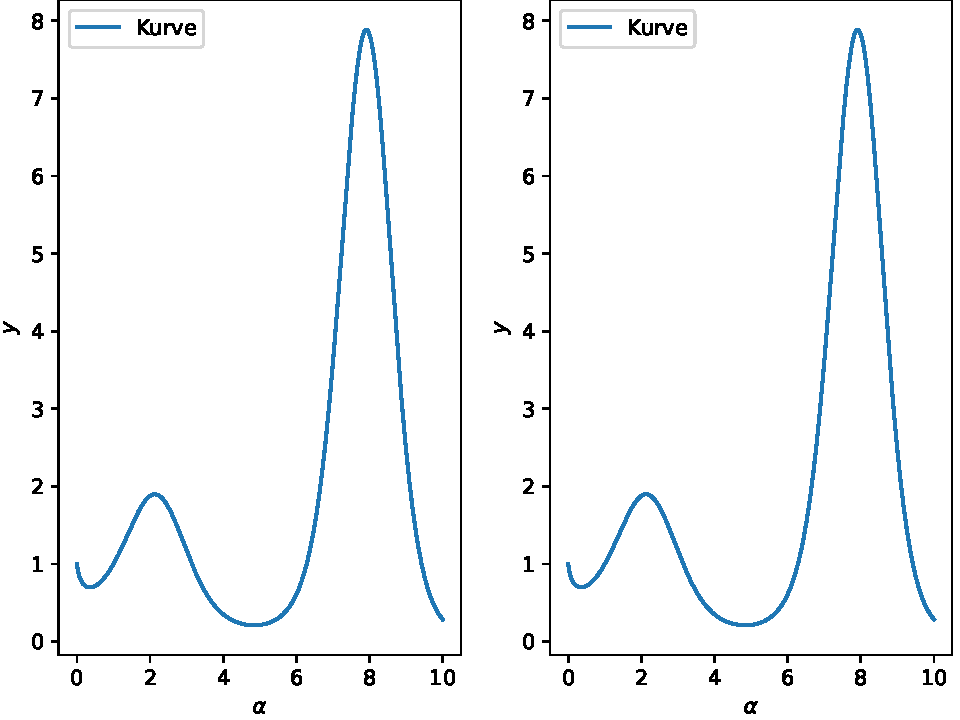
\includegraphics{plot.pdf}
  \caption{Periodendauer der beiden Pendel mit einer Pendellänge von 70 cm.}
  \label{fig:plot}
\end{figure}


%Siehe \autoref{fig:plot}! blaaaaaaaaaaaaaaaaaaaaa
